%%%
% Plantilla de Memoria
% Modificación de una plantilla de Latex de Nicolas Diaz para adaptarla 
% al castellano y a las necesidades de escribir informática y matemáticas.
%
% Editada por: Mario Román
%
% License:
% CC BY-NC-SA 3.0 (http://creativecommons.org/licenses/by-nc-sa/3.0/)
%%%

%%%%%%%%%%%%%%%%%%%%%%%%%%%%%%%%%%%%%%%%%
% Thin Sectioned Essay
% LaTeX Template
% Version 1.0 (3/8/13)
%
% This template has been downloaded from:
% http://www.LaTeXTemplates.com
%
% Original Author:
% Nicolas Diaz (nsdiaz@uc.cl) with extensive modifications by:
% Vel (vel@latextemplates.com)
%
% License:
% CC BY-NC-SA 3.0 (http://creativecommons.org/licenses/by-nc-sa/3.0/)
%
%%%%%%%%%%%%%%%%%%%%%%%%%%%%%%%%%%%%%%%%%

%----------------------------------------------------------------------------------------
%	PAQUETES Y CONFIGURACIÓN DEL DOCUMENTO
%----------------------------------------------------------------------------------------
%%% Configuración del papel.
% microtype: Tipografía.
% mathpazo: Usa la fuente Palatino.
\documentclass[a4paper, 11pt]{article}
\usepackage[protrusion=true,expansion=true]{microtype}
\usepackage{mathpazo}

\usepackage{fancyvrb}

% redefine \VerbatimInput
\RecustomVerbatimCommand{\VerbatimInput}{VerbatimInput}%
{fontsize=\footnotesize,
	%
	frame=lines,  % top and bottom rule only
	framesep=2em, % separation between frame and text
	rulecolor=\color{Gray},
	%
	label=\fbox{\color{Black}data.txt},
	labelposition=topline,
	%
	commandchars=\|\(\), % escape character and argument delimiters for
	% commands within the verbatim
	commentchar=*        % comment character
}


\usepackage{movie15}


% Indentación de párrafos para Palatino
\setlength{\parindent}{0pt}
  \parskip=8pt
\linespread{1.05} % Change line spacing here, Palatino benefits from a slight increase by default




%%% Castellano.
% noquoting: Permite uso de comillas no españolas.
% lcroman: Permite la enumeración con numerales romanos en minúscula.
% fontenc: Usa la fuente completa para que pueda copiarse correctamente del pdf.
\usepackage[spanish,es-noquoting,es-lcroman]{babel}
\usepackage[utf8]{inputenc}
\usepackage[T1]{fontenc}
\selectlanguage{spanish}




%%% Gráficos
\usepackage{graphicx} % Required for including pictures
\usepackage{wrapfig} % Allows in-line images
\usepackage[usenames,dvipsnames]{color} % Coloring code
\usepackage{graphicx}

%%% Matemáticas
\usepackage{amsmath}


%%% Bibliografía
\makeatletter
\renewcommand\@biblabel[1]{\textbf{#1.}} % Change the square brackets for each bibliography item from '[1]' to '1.'
\renewcommand{\@listI}{\itemsep=0pt} % Reduce the space between items in the itemize and enumerate environments and the bibliography


%% codigo

%%% CÓDIGO
 \usepackage{listings}
\usepackage{courier}
\lstset{
	basicstyle=\footnotesize\ttfamily, % Standardschrift
	numbers=left,               % Ort der Zeilennummern
	numberstyle=\tiny,          % Stil der Zeilennummern
	stepnumber=1,               % Abstand zwischen den Zeilennummern
	numbersep=5pt,              % Abstand der Nummern zum Text
	tabsize=2,                  % Groesse von Tabs
	extendedchars=true,         %
	breaklines=true,            % Zeilen werden Umgebrochen
	keywordstyle=\color{red},
	frame=b,         
	%        keywordstyle=[1]\textbf,    % Stil der Keywords
	%        keywordstyle=[2]\textbf,    %
	%        keywordstyle=[3]\textbf,    %
	%        keywordstyle=[4]\textbf,   \sqrt{\sqrt{}} %
	stringstyle=\color{white}\ttfamily, % Farbe der String
	showspaces=false,           % Leerzeichen anzeigen ?
	showtabs=false,             % Tabs anzeigen ?
	xleftmargin=17pt,
	framexleftmargin=17pt,
	framexrightmargin=5pt,
	framexbottommargin=4pt,
	%backgroundcolor=\color{lightgray}
	showstringspaces=false      % Leerzeichen in Strings anzeigen ?        
	literate=
	{á}{{\'a}}1 {é}{{\'e}}1 {í}{{\'i}}1 {ó}{{\'o}}1 {ú}{{\'u}}1
	{Á}{{\'A}}1 {É}{{\'E}}1 {Í}{{\'I}}1 {Ó}{{\'O}}1 {Ú}{{\'U}}1
	{à}{{\`a}}1 {è}{{\`e}}1 {ì}{{\`i}}1 {ò}{{\`o}}1 {ù}{{\`u}}1
	{À}{{\`A}}1 {È}{{\'E}}1 {Ì}{{\`I}}1 {Ò}{{\`O}}1 {Ù}{{\`U}}1
	{ä}{{\"a}}1 {ë}{{\"e}}1 {ï}{{\"i}}1 {ö}{{\"o}}1 {ü}{{\"u}}1
	{Ä}{{\"A}}1 {Ë}{{\"E}}1 {Ï}{{\"I}}1 {Ö}{{\"O}}1 {Ü}{{\"U}}1
	{â}{{\^a}}1 {ê}{{\^e}}1 {î}{{\^i}}1 {ô}{{\^o}}1 {û}{{\^u}}1
	{Â}{{\^A}}1 {Ê}{{\^E}}1 {Î}{{\^I}}1 {Ô}{{\^O}}1 {Û}{{\^U}}1
	{œ}{{\oe}}1 {Œ}{{\OE}}1 {æ}{{\ae}}1 {Æ}{{\AE}}1 {ß}{{\ss}}1
	{ű}{{\H{u}}}1 {Ű}{{\H{U}}}1 {ő}{{\H{o}}}1 {Ő}{{\H{O}}}1
	{ç}{{\c c}}1 {Ç}{{\c C}}1 {ø}{{\o}}1 {å}{{\r a}}1 {Å}{{\r A}}1
	{€}{{\euro}}1 {£}{{\pounds}}1 {«}{{\guillemotleft}}1
	{»}{{\guillemotright}}1 {ñ}{{\~n}}1 {Ñ}{{\~N}}1 {¿}{{?`}}1   
}


\lstloadlanguages{% Check Dokumentation for further languages ...
%[Visual]Basic
%Pascal
%C
C++
%%XML
%%HTML
%Java
}
%\DeclareCaptionFont{blue}{\color{blue}} 

%\captionsetup[lstlisting]{singlelinecheck=false, labelfont={blue}, textfont={blue}}
\usepackage{caption}
\DeclareCaptionFont{white}{\color{white}}
\DeclareCaptionFormat{listing}{\colorbox[cmyk]{0.43, 0.35, 0.35,0.01}{\parbox{\textwidth}{\hspace{15pt}#1#2#3}}}
\captionsetup[lstlisting]{format=listing,labelfont=white,textfont=white, singlelinecheck=false, margin=0pt, font={bf,footnotesize}
}

%% cosas 

\usepackage[margin=1in]{geometry}

\usepackage{times}


%% colorear titulos
\usepackage{titlesec}
\titleformat{\section}
{\color{rojizo}\normalfont\Large\bfseries}
{\color{Black}\thesection}{1em}{}


%% ENLACES 
\usepackage{hyperref}
\hypersetup{
	colorlinks   = true,    % Colours links instead of ugly boxes
	urlcolor     = black,    % Colour for external hyperlinks
	linkcolor    = black, %BurntOrange,    % Colour of internal links
	citecolor    = black      % Colour of citations
}


%% CREAR DIAGRAMAS 

\usepackage{tikz}

%% rodear figura de texto
\usepackage{graphicx,wrapfig,lipsum}
 %% comentarios multilinea
\usepackage{verbatim}

\definecolor{darkGray}{gray}{0.05}
\usepackage{animate}
\definecolor{rojizo}{RGB}{217, 83, 79}


%----------------------------------------------------------------------------------------
%	DOCUMENTO
%----------------------------------------------------------------------------------------

\begin{document}
	



%\maketitle % Print the title section

%% Resumen (Descomentar para usarlo)
\renewcommand{\abstractname}{Resumen} % Uncomment to change the name of the abstract to something else
%\begin{abstract}
% Resumen aquí
%\end{abstract}

%% Palabras clave
%\hspace*{3,6mm}\textit{Keywords:} lorem , ipsum , dolor , sit amet , lectus % Keywords
%\vspace{30pt} % Some vertical space between the abstract and first section

\color{darkGray}
%% Índice
{\parskip=2pt
  \tableofcontents
}
\section{CUESTIONES}
\subsection{El concepto de juego. Elementos y clasificación de los juegos.}
\subsection{El algoritmo minmax. Componentes y funcionamiento.}
\subsection{Modelos de representación del conocimiento.}
\subsection{Modelos de conocimiento heredable. Herencia.}
\subsection{Paradigmas de aprendizaje.}
\subsection{Aprendizaje inductivo. Empleo de árboles de decisión en aprendizaje inductivo.}
\pagebreak
\section{RESPUESTAS}
\subsection{El concepto de juego. Elementos y clasificación de los juegos.}
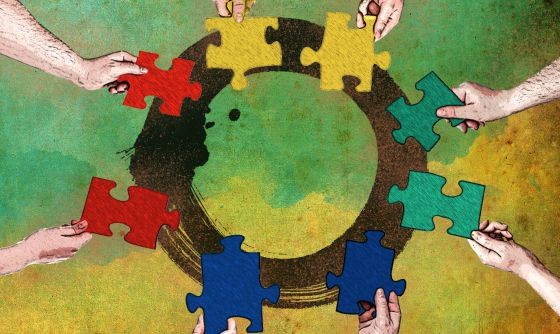
\includegraphics[width=\textwidth]{juegos.jpg} 

Un juego es cualquier situación de decisión con \textbf{varios agentes} (llamados jugadores) gobernada por un \textbf{conjunto de reglas} y con un resultado bien definido, caracterizada porque \textbf{ninguno de los jugadores con su sola actuación puede determinar el resultado} (independencia estratégica).
Lo que caracteriza a un juego es el \textbf{número de jugadores}, la \textbf{información con que cuentan los jugadores} (perfecta o imperfecta), la \textbf{existencia o no de movimientos de azar}, el \textbf{orden de actuación de los jugadores}, los \textbf{repartos de beneficios} (que determinan si se trata de juegos de suma nula o no nula) y la \textbf{existencia o no de pagos colaterales} (equilibrio de Nash). Respecto a los elementos de un juego: intervienen, además de los juadores, las distintas estrategias que estos pueden seguir (que están condicionada por las reglas que rigen el desarrollo del juego) y los pagos o beneficios que obtendrá cada jugador en función de la estrategia que utilice cada uno. (a cada tupla de estrategias, una por jugador, le corresponde una tupla de beneficios obtenidos, uno por jugador). 

\pagebreak
\subsection{El algoritmo minmax. Componentes y funcionamiento.}
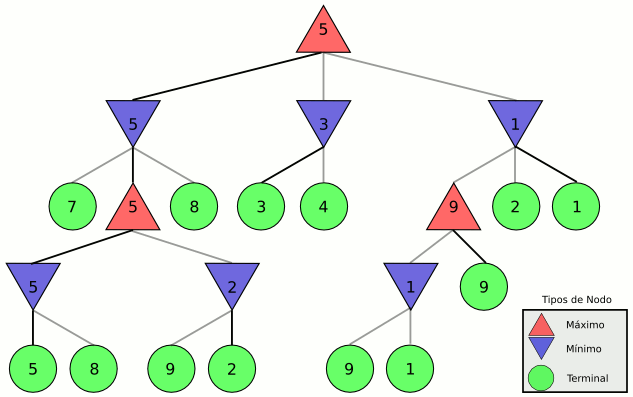
\includegraphics[width=\textwidth]{minmax.png} 
El algoritmo minmax es un algoritmo usado para tomar decisiones óptimas en \textbf{juegos bipersonales competitivos.} Los componentes del algoritmo son:
\begin{description}

\item [Los jugadores:]a los que se denominará Max y Min, siendo Max el jugador que comienza la partida.
\item [Estado inicial:]que identifica la situación en que comienza el juego y determina las posibles estrategias de los jugadores
\item [Función sucesor:]determina, para cada movimiento legal, el estado al que conduce.
\item [Función de utilidad:]determina los resultados de la partida en los nodos terminales. Los resultados favorables a Max serán positivos y los favorables a Min, negativos. En caso de empate el resultado será 0.
\item [Función terminal:]determina si un nodo es o no terminal (si supone el fin de la partida).
\end{description}

El algoritmo calcula la acción que conduce al mejor resultado para el jugador. En el caso de Max conduce al mayor valor posible y en el caso de Min, al menor (que decir al peor resultado para Max y el mejor para Min) Para ello, genera un \textbf{árbol de juego} con todos los estados posibles que resultan de las distintas acciones de los jugadores hasta obtener los nodos terminales, calcula los valores de dichos nodos terminales utilizando la función de utilidad y los de los nodos no terminales utilizando los valores de sus hijos. El algoritmo asignara a cada nivel del árbol un rol Max o Min en función de a qué jugador le corresponde actuar y asigna el mayor (o menor) valor de los nodos de los hijos dependiendo de si se trata de una decisión que toma Max o Min (Max pretende maximizar el valor de los nodos y Min minimizarlo). Se trata de una exploración primero en profundidad en la que se debe explorar todo el árbol por lo que el tiempo necesario para calcular el árbol de juego de un caso complejo puede ser inabarcable. Por esta razón, el algoritmo de por sí no nos resulta útil. No obstante, es la base de algoritmos más complejos como la poda alpha-beta.

\subsection{Modelos de representación del conocimiento.}
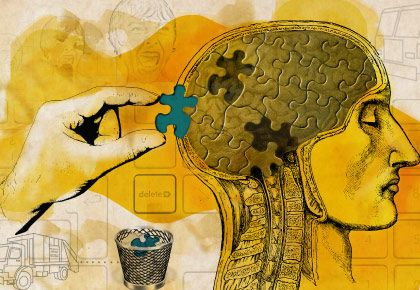
\includegraphics[width=\textwidth]{representacion.jpg} 
Un modelo de representación del conocimiento es un formalismo simbólico empleado para expresar el conocimiento, un modelo mental que se caracteriza por la semántica con que representa ciertos aspectos del dominio o universo con el que un sistema software pueda trabajar. Entre sus características está aquello ue puede representar (representación icónica o representación descriptiva), la granularidad de la representación (nivel de detalle), el tipo de descripciones (intensionales o extensionales), la representación del metaconocimiento (conocimiento sobre el propio conocimiento, independiente del mismo) y la jerarquización de objetos y herencia. 
Así, encontramos modelos inspirados por la psicología como:
\begin{itemize}
 \item Los modelos de conducta o reglas de producción, que son reglas de inferencia del tipo si ocurre A, entonces ocurre B.
 \item Los modelos de razonamiento o lógicas, que son lenguajes formales con símbolos, semántica y sintaxis que permiten representar el conocimiento y formular inferencias que permitan obtener nuevo conocimiento a partir de conocimiento previo gracias a la teoría de la demostración, siendo la lógica de proposiciones y la lógica de predicados las dos más simples.
 \item Los modelos de memoria, que representan el conocimiento como conjuntos de elementos y relaciones entre ellos. Bien con modelos de conocimiento relacional simple (ficheros y bases de datos, con relaciones expresables mediante tablas) que requerirán de un motor de inferencia para generar nuevo conocimiento, o bien con modelos de conocimiento heredable (que jerarquizan el conocimiento), utilizando redes asociativas (semánticas, de clasificación o causales), marcos, frames, representación orientada a objetos...
 \end{itemize}

Además, existen otros modelos y problemas en la representación del conocimiento como la necesidad de representación del sentido común, la organización jerárquica del conocimiento, el razonamiento temporal o la lógica difusa.
 
\subsection{Modelos de conocimiento heredable. Herencia.}
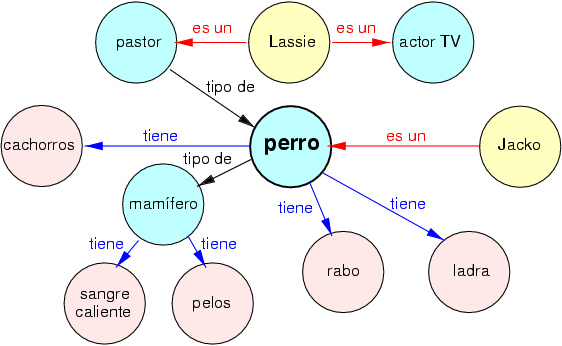
\includegraphics[width=\textwidth]{racimo.png} 
Los modelos de conocimiento heredable se basan en la jerarquización del conocimiento de forma que se puedan inferir características o atributos de ciertos elementos a partir de otras ya conocidas. Por ejemplo, un marco o frame es una estructura de datos formada por un conjunto de campos que se asocian por lo general a atributos que sirven para identificar los marcos. Se utilizan para tareas de reconocimiento ya que la información contenida en un marco puede hacer que se activen otros marcos conectados con los primeros, dando lugar así a una red de activación que permite predecir y explicar la información que deriva de los marcos activados inicialmente. Al conocimiento que surge de este mecanismo se le suele denominar herencia o reconocimiento descendiente porque se determinan propiedades desconocidas de ciertos elementos a partir de otras ya conocidas que las encapsulan. Por ejemplo, si un frame `pájaro' contiene el campo `movimiento: volar', y otro frame, `periquito', contiene el campo `tipo: pájaro' entonces se puede inferir que el periquito puede volar a no ser que el frame `periquito' contenga un campo `movimiento' con un valor distinto a `volar'.

Por otro lado, las llamadas redes asociativas están formadas por nodos que representan un concepto o una proposición, enlazados entre sí de forma que se representan relaciones de inclusión, pertenencia o causalidad o bien a categorías gramaticales (verbo, sujeto, complemento, etc.) Algunos tipos de redes asociativas son:
\begin{itemize}
	\item redes semánticas: son las destinadas a representar o a comprender el lenguaje natural.
	\item redes de clasificación: clasificaciones de objetos o conceptos según sus características propias (con herencia).
	\item redes causales: son las que llevan asociadas una relación de influencia o causa entre los nodos que las forman (el hecho representado por el nodo A provoca el hecho representado por el nodo B y por eso ambos nodos están relacionados.)
\end{itemize}


\subsection{Paradigmas de aprendizaje.}
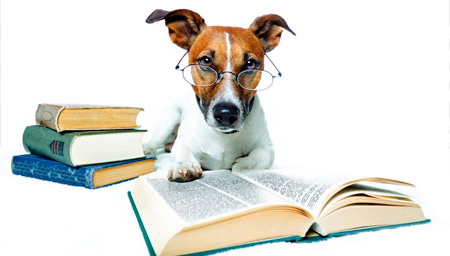
\includegraphics[width=0.60\textwidth]{perro.jpg} 

En el campo del aprendizaje automático encontramos, principalmente, los siguientes paradigmas de aprendizaje:
\begin{description}
	\item[Aprendizaje memorístico] surge cuando el aprendizaje consta de asociaciones arbitrarias o cuando el sujeto lo hace de forma arbitraria. Los datos se almacenan sin tratar de comprenderlos o de inferirlos a partir de otros ya conocidos y de forma repetitiva. Por ejemplo, si un sistema recibe, ante una determinada acción en cierta circunstancia, una respuesta desventajosa, puede `memorizar' que esa acción da malos resultados y, si esos malos resultados se repiten en el tiempo, concluir (aprender) que esa no es una acción adecuada para dicha situación.
	\item[Aprendizaje deductivo] consiste en aplicar la deducción para obtener descripciones generales a partir de un ejemplo de concepto y su explicación. Es decir, es la obtención de nuevo conocimiento a partir de conocimientos que ya se poseen. También es el razonamiento artificial (dar una explicación a un evento observado a partir de conocimientos previos y crear así nuevo conocimiento.)
	\item[Aprendizaje analítico, Basado en explicaciones] Construir una explicación para cada ejemplo en relación con un concepto dado y generalizar la explicación de modo que pueda emplearse en el futuro. Los métodos analíticos usan el conocimiento primario para deducir las hipótesis generales. Aquí, se buscan hipótesis generales que se ajusten al conocimiento primario mientras se cubren los datos observados.
	\item[Aprendizaje analógico] se buscan soluciones a problemas nuevos encontrando similitudes con problemas ya conocidos y adaptando sus soluciones. Se basa en la idea de que, si dos situaciones son similares en algún aspecto, entonces también pueden serlo en otros. 
	\item[Aprendizaje inductivo]  se trata de aprender un concepto o una clasificación a partir de ejemplos y contraejemplos. Se formulan hipótesis mediante la búsqueda de regularidades en unos ejemplos de `entrenamiento' observados previamente (ejemplos) y se aceptan o rechazan dichas hipótesis con la aparición de nuevos ejemplos.
\end{description}

Tipos de aprendizaje según su conocimiento:

\begin{description}
	\item[Supervisado] Se dispone de un profesor/supervisor que proporciona una salida deseable para cada entrada percibida, ya sea una clase o un valor a aproximar(clasificación vs regresión).
	\item[No supervisado] No se dispone de una salida deseada cada entrada, sino que se busca agrupar/clasificar los datos en función de ciertas características(medida de distancia)
	\item[Refuerzo] Se aprende (sin supervisor) a partir de la información obtenida al realizar procesos de ensayo-error en los que se obtienen “señales” de beneficio/coste.
\end{description}

\subsection{Aprendizaje inductivo. Empleo de árboles de decisión en aprendizaje inductivo.}
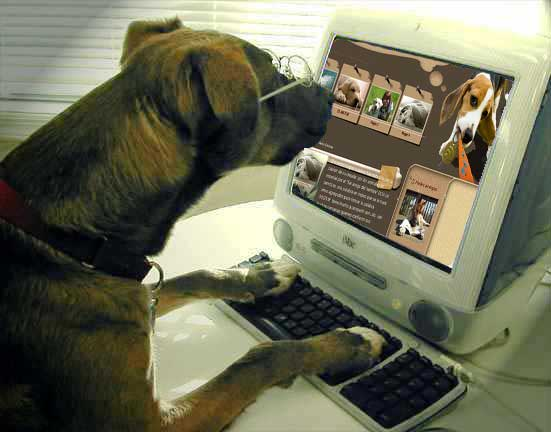
\includegraphics[width=\textwidth]{perrete.jpg} 

Se trata de aprender un concepto o una clasificación a partir de ejemplos y contraejemplos. El objetivo es aprender la función f.
Un ejemplo es un par (x,f(x)).
Dada una colección de ejemplos de f, devolver una función h( hipótesis ) que aproxime a f.
La razón por el cual el aprendizaje es difícil es porque no es fácil determinar si una función h es una buena aproximación de h. Una buena hipótesis estará bien generalizada si puede predecir ejemplos que no se conocen.

Un árbol de decisión se puede utilizar para el aprendizaje inductivo si toma como entrada un objeto o una situación descrita a través de un conjunto de atributos y devuelve una decisión(valor previsto de la salida dada por la entrada).
Los atributos de entradas y salida pueden ser discretos o continuos.
Aprender una función de valores discretos se denomina clasificación.
Aprender una función continua se denomina regresión.
Resumiendo, un árbol de decisión, desarrolla una secuencia de test para poder alcanzar una decisión.
Cada nodo corresponde con un test sobre el valor de una de las propiedades, y las ramas que salen de cada nodo están etiquetadas con los posibles valores de dicha propiedad. Cada nodo hoja representa el valor que ha de ser devuelto si dicho nodo hoja es alcanzado.



\end{document}